%!TEX root = ../../da.tex

\chapter{Heat Flux for Semi-Local Machine-Learning Potentials}
\label{ch:si-heat_flux}


\section{Testing Forces and Stress}
\label{sec:si-glp_testing}

In order to verify the approach described in \cref{ch:glps}, and to test the \glpc framework, potential energy, forces, and stress for the Lennard-Jones potential were compared with the implementation in \gls{ase}, where derivatives are computed analytically, and all operations are performed in double precision arithmetic.

The experiment consists of computing these properties for \num{100} randomly perturbed simulation cells of Lennard-Jones argon as defined in \cref{sec:lj-ar}, starting from an $8\times8\times8$ supercell of the face-centred cubic primitive cell with lattice parameter $\qty{3.72}{\angstrom}$ and angle $\qty{60}{\degree}$.

Positions are then perturbed slightly, with perturbations drawn from a normal distribution with $\sigma{=}\qty{0.01}{\angstrom}$; a random strain with each component drawn from a uniform distribution over $[-0.1, 0.1]$ is also applied.
For each such structure, energy, forces, and stress are computed using a number of different approaches
\begin{itemize}[itemsep=0pt,topsep=0.5\baselineskip]
	\item The analytical implementation in \gls{ase},
	\item \texttt{glp} implementation where $\graph$ is constructed using the \mic in \emph{fractional} coordinates,
	\item \texttt{glp} implementation where $\graph$ is constructed using the \mic using explicit offsets,
	\item \texttt{glp} implementation using the \scare{unfolded} graph construction where no \mic is applied,
	\item Finite differences using a \texttt{glp} calculator, where the displacements have been chosen to minimise the deviation from \gls{ase}, see \cref{fig:si-glps_lj_stress_fd_convergence_32}.
\end{itemize}
For the forces, we compare approaches where gradients are computed with respect to positions directly, and those where gradients are compared with respect to edges.
For the stress, \cref{eq:glp_stress_strain_direct,eq:glp_stress_strain_edges,eq:glp_stress_strain_unf,eq:glp_stress_sc_basis,eq:glp_stress_edges,eq:glp_stress_bulk} are compared, using the graph construction required to produce the correct stress.

\Cref{tab:si-glps_lj_forces_error_32,tab:si-glps_lj_forces_error_64,tab:glps_lj_stress_error_32,tab:si-glps_lj_stress_error_64} show the result.
For the forces, all \mic-based implementation approaches are equivalent and in excellent agreement with the analytical implementation.
For the stress, all given formulations are found to be equivalent as well. In single precision arithmetic, the \ad-based implementations are more accurate than finite differences, in double precision, errors are similar. 

% \begin{table}
%     \caption{
%     Comparison of deviations in energy for different \glp implementations of the Lennard-Jones potential, compared with the implementation in \gls{ase}.
%     Results are shown for single precision arithmetic.
%     }
%     \begin{tabular}{l | r r r r}
\toprule
             Comment  &  \acs{mae} in \unit{eV}  &  \acs{maxae} in \unit{eV}  &  \acs{mape} in \unit{\percent}  &  \acs{maxape} in \unit{\percent} \\ 
\midrule
  \acs{mic} (offset)  &        \num{1.70e-06}  &        \num{5.11e-06}  &        \num{3.88e-06}  &        \num{1.17e-05} \\ 
   \acs{mic} (frac.)  &        \num{1.71e-06}  &        \num{5.78e-06}  &        \num{3.92e-06}  &        \num{1.32e-05} \\ 
            Unfolded  &        \num{1.83e-06}  &        \num{5.27e-06}  &        \num{4.18e-06}  &        \num{1.21e-05} \\ 
\bottomrule
\end{tabular}

%     \label{tab:si-glps_lj_energy_error_32}
% \end{table}

\begin{table}
    \caption{
    Comparison of deviations in forces for different \glp implementations of the Lennard-Jones potential, compared with the implementation in \gls{ase}.
    Results are shown for single precision arithmetic.
    }
    \begin{tabular}{l l | r r}
\toprule
             Comment  &                 Grads  &  \acs{mae} in \unit{eV\per\angstrom}  &  \acs{maxae} in \unit{eV\per\angstrom} \\ 
\midrule
  \acs{mic} (offset)  &                 edges  &        \num{2.72e-07}  &        \num{2.07e-06} \\ 
   \acs{mic} (frac.)  &                 edges  &        \num{2.58e-07}  &        \num{1.88e-06} \\ 
  \acs{mic} (offset)  &                direct  &        \num{2.72e-07}  &        \num{2.07e-06} \\ 
   \acs{mic} (frac.)  &                direct  &        \num{2.58e-07}  &        \num{1.89e-06} \\ 
            Unfolded  &                direct  &        \num{1.76e-07}  &        \num{1.64e-06} \\ 
\bottomrule
\end{tabular}

    \label{tab:si-glps_lj_forces_error_32}
\end{table}
\vspace{2\baselineskip}

\begin{table}
    \caption{
    Comparison of deviations in forces for different \glp implementations of the Lennard-Jones potential, compared with the implementation in \gls{ase}.
    Results are shown for double precision arithmetic.
    }
    \begin{tabular}{l l | r r}
\toprule
             Comment  &                 Grads  &  \acs{mae} in \unit{eV\per\angstrom}  &  \acs{maxae} in \unit{eV\per\angstrom} \\ 
\midrule
  \acs{mic} (offset)  &                 edges  &        \num{3.58e-10}  &        \num{2.21e-09} \\ 
   \acs{mic} (frac.)  &                 edges  &        \num{3.58e-10}  &        \num{2.21e-09} \\ 
  \acs{mic} (offset)  &                direct  &        \num{3.58e-10}  &        \num{2.21e-09} \\ 
   \acs{mic} (frac.)  &                direct  &        \num{3.58e-10}  &        \num{2.21e-09} \\ 
            Unfolded  &                direct  &        \num{3.58e-10}  &        \num{2.21e-09} \\ 
\bottomrule
\end{tabular}

    \label{tab:si-glps_lj_forces_error_64}
\end{table}
\vspace{2\baselineskip}

\begin{table}
    \caption{
    Error in stress for Lennard-Jones argon,
    comparing different formulations, as well as finite differences, with a baseline implementation in \gls{ase}.
    % , where derivatives are obtained analytically.
    Results are shown for double precision arithmetic, and for $\stress \cdot V$ in place of $\stress$.
    }
    \begin{tabular}{l | r r r r}
\toprule
            Equation  &  \acs{mae} in \unit{eV}  &  \acs{maxae} in \unit{eV}  &  \acs{mape} in \unit{\percent}  &  \acs{maxape} in \unit{\percent} \\ 
\midrule
          Fin. diff.  &        \num{1.13e-06}  &        \num{7.49e-06}  &        \num{1.18e-04}  &        \num{8.55e-03} \\ 
\ref{eq:glp_stress_strain_direct}  &        \num{3.15e-06}  &        \num{1.04e-05}  &        \num{3.69e-04}  &        \num{2.72e-02} \\ 
\ref{eq:glp_stress_strain_edges}  &        \num{3.15e-06}  &        \num{1.04e-05}  &        \num{3.69e-04}  &        \num{2.72e-02} \\ 
\ref{eq:glp_stress_strain_unf}  &        \num{3.15e-06}  &        \num{1.04e-05}  &        \num{3.69e-04}  &        \num{2.72e-02} \\ 
\ref{eq:glp_stress_sc_basis}  &        \num{3.15e-06}  &        \num{1.04e-05}  &        \num{3.69e-04}  &        \num{2.72e-02} \\ 
\ref{eq:glp_stress_edges}  &        \num{3.15e-06}  &        \num{1.04e-05}  &        \num{3.69e-04}  &        \num{2.72e-02} \\ 
\ref{eq:glp_stress_bulk}  &        \num{3.15e-06}  &        \num{1.04e-05}  &        \num{3.69e-04}  &        \num{2.72e-02} \\ 
\bottomrule
\end{tabular}

    \label{tab:si-glps_lj_stress_error_64}
\end{table}


% \clearpage

\begin{figure}
  \includegraphics[width=\textwidth]{img/plot/gk/si-lj_stress_fd_convergence.pdf}
  \caption{
  \gls{mae} of stress obtained via finite differences compared to the analytical implementation for different choices of displacement, for single and double precision. The minimum is marked with a dot.
  }
  \label{fig:si-glps_lj_stress_fd_convergence_32}
\end{figure}


% \begin{table}
%     \caption{
%     Comparison of deviations in stress for different \glp implementations of the Lennard-Jones potential, compared with the implementation in \gls{ase}, where forces are obtained analytically, and the stress obtained via the finite difference method.
%     Results are shown for single precision arithmetic.
%     }
%     \begin{tabular}{l | r r r r}
\toprule
            Equation  &  \acs{mae} in \unit{eV}  &  \acs{maxae} in \unit{eV}  &  \acs{mape} in \unit{\percent}  &  \acs{maxape} in \unit{\percent} \\ 
\midrule
          Fin. diff.  &        \num{7.70e-04}  &        \num{4.18e-03}  &        \num{1.04e-01}  &        \num{5.30e+00} \\ 
\ref{eq:glp_stress_strain_direct}  &        \num{1.19e-05}  &        \num{6.54e-05}  &        \num{1.79e-03}  &        \num{7.35e-02} \\ 
\ref{eq:glp_stress_strain_edges}  &        \num{8.25e-06}  &        \num{4.11e-05}  &        \num{1.27e-03}  &        \num{6.75e-02} \\ 
\ref{eq:glp_stress_strain_unf}  &        \num{9.17e-06}  &        \num{4.46e-05}  &        \num{1.36e-03}  &        \num{4.39e-02} \\ 
\ref{eq:glp_stress_sc_basis}  &        \num{1.18e-05}  &        \num{6.44e-05}  &        \num{1.79e-03}  &        \num{7.19e-02} \\ 
\ref{eq:glp_stress_edges}  &        \num{8.22e-06}  &        \num{4.16e-05}  &        \num{1.27e-03}  &        \num{6.59e-02} \\ 
\ref{eq:glp_stress_bulk}  &        \num{9.16e-06}  &        \num{4.51e-05}  &        \num{1.37e-03}  &        \num{4.92e-02} \\ 
\bottomrule
\end{tabular}

%     \label{tab:si-glps_lj_stress_error_32}
% \end{table}

% \clearpage

% \begin{figure}
%   \includegraphics[width=\textwidth]{img/plot/gk/si-lj_stress_fd_convergence_32.pdf}
%   \caption{
%   \gls{mae} of stress obtained via finite differences compared to the analytical implementation for different choices of displacemen, for single precision. The minimum is marked with a red star, other choices with black ones.
%   }
%   \label{fig:si-glps_lj_stress_fd_convergence_32}
% \end{figure}


% \begin{figure}
%   \includegraphics[width=\textwidth]{img/plot/gk/si-lj_stress_fd_convergence_64.pdf}
%   \caption{
%   \gls{mae} of stress obtained via finite differences compared to the analytical implementation for different choices of displacement, for double precision. The minimum is marked with a red star, other choices with black ones.
%   }
%   \label{fig:si-glps_lj_stress_fd_convergence_64}
% \end{figure}

% \clearpage
\section{Lennard-Jones Argon}
\label{sec:lj-ar}

The following parameters are used to model Lennard-Jones argon, following reference~\cite{mk2004t}:
$\sigma{=}\qty{3.405}{\angstrom}$, $\epsilon{=}\qty{0.01042}{eV}$, $\cutoff{=}\qty{10.5}{\angstrom}$, $\onset{=}\qty{9.0}{\angstrom}$,
where $\onset$ is the \scare{onset} parameter of the cutoff function $\fcutoff$ that ensures that forces smoothly decay to zero as the cutoff radius $\cutoff$ is approached.

This cutoff function is multiplied onto $U(r_{ij})$ and is defined as 
\begin{equation}
	\fcutoff(r) = \begin{cases}
		1 &  \text{for } r < \onset \\
		\frac{(\cutoff^2 - r^2)^2 (\cutoff^2 + 2 r^2 - 3 \onset^2)}{(\cutoff^2 - \onset^2)^3} & \text{for } \onset \leq r \leq \cutoff \\
		0 &  \text{for } r > \cutoff \, .
	\end{cases}
\end{equation}

%%%%%%% Unfolding
% \clearpage
\section{Efficient Unfolding}
\label{sec:si-unf_imp}

In order to implement the unfolded heat flux, we must be able to efficiently construct $\Runf$ from $\Rsc$ and $\Basis$. We present a simple and vectorisable approach.

\newthought{Consider our objective:} For each position $\Rsc$, we must determine \emph{(a)} whether it requires replication at all, and \emph{(b)} if yes, in which directions. Both can be achieved by breaking the task down into a series of steps.
\begin{enumerate}[itemsep=0pt,topsep=0.5\baselineskip]
  \item For each position $i \in \Rsc$, determine whether it lies within $\effcutoff$ of any of the six faces of the simulation cell. If this is the case, $i$ is said to have a collision with that boundary. (See \cref{sec:si-unf-triclinic} for a discussion of the non-orthorhombic case.).
  % In any case, the resulting comparisons are straightforward checks on arrays that can be readily vectorised with \texttt{numpy}.
  \item From the resulting collisions, compute which replicas of each $i$ must be constructed. There are 26 possibilities: 
  \begin{enumerate}
    \item If $i$ collides with a boundary, it is replicated in the opposite direction of that boundary (6 cases).
    \item If it collides with two, it collides with an edge and must therefore also be replicated diagonally (12 cases).
    \item If it collides with three boundaries, it collides with a corner and must also be replicated diagonally (8 cases).
  \end{enumerate}
  \item Construct the replicas from this prescription.
\end{enumerate}
% An instructive example of this is given in \cref{fig:hfi-unfolding}.

Separating steps two and three allows the determination of the unfolding outside the computational graph, and also enables the caching of results: by increasing the cutoff used for unfolding by a tolerance $\skin$, it must only be recomputed if the distance of any position to the boundary changes by more than $\skin/2$. While the unfolding is typically not a bottleneck in the systems investigated in this work, this caching also avoids oscillations of atoms close to the cutoff boundary, which in turn avoids cache misses in the neighbourlist construction.
% , which can be computationally expensive.

\section{Unfolding for Non-Orthorhombic Systems}
\label{sec:si-unf-triclinic}

The simulation cell is spanned by $\Basis = (\basis_1, \basis_2, \basis_3)$, forming a parallelpepiped. Our task is to determine the sets of points within\footnote{We assume that in a pre-processing step, every positions has been wrapped into the simulation cell.} this parallelpepiped that lie within $\effcutoff$ of each of the six faces. There are two straightforward approaches to solving this problem: We can project all positions onto the surface normals of the faces, directly measuring the distances to the faces, or we can transition to fractional coordinates, where distances to the faces can be obtained by inspecting the components of the resulting coordinates. We choose the former of these two equivalent approaches.
% , prefering a real-space approach with a direct geometric interpretation. 

As a first step, we therefore obtain the surface normals $\nsurf_1, \nsurf_2, \nsurf_3$, which are simply the normalised reciprocal lattice vectors.\footnote{
  In particular
  \begin{align*}
    \nsurf_1 &\propto \basis_2 \times \basis_3 \\
    \nsurf_2 &\propto \basis_3 \times \basis_1 \\
    \nsurf_3 &\propto \basis_1 \times \basis_2 \, .
\end{align*}
}
The surface normals are oriented inwards, in the direction of, but in general not parallel to, the basis vector that shares the same index.

Then, we compute the distances $d_i$ between opposite faces by projecting the basis vectors onto the surface normals, $d_\alpha = \basis_\alpha \cdot \nsurf_\alpha$. 
Similarly, for each position $\R_i$ we compute the components along the surface normals, yielding projected positions $r'^{\alpha}_i = \R_i \cdot \nsurf_\alpha$.
Now, collisions with the two surfaces in direction $\alpha$ can be detected by checking $r'^{\alpha}_i \leq \effcutoff$ or $r'^{\alpha}_i \geq d_\alpha - \effcutoff$.

% This approach requires elementary linear algebra operations and boolean checks that can be readily vectorised across arrays, making it highly efficient.

\section{Size of Unfolded System}
\label{sec:si-unfolding_n}

\begin{marginfigure}
  \centering
  
  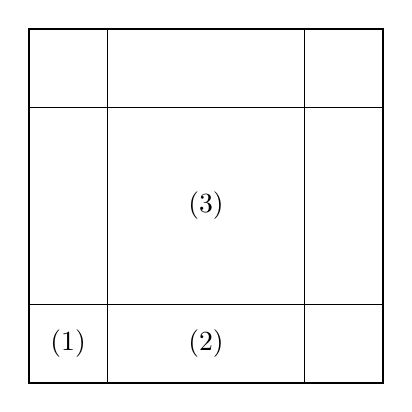
\begin{tikzpicture}[
      x = 1cm,
      y = 1cm,
  ]

  \draw [solid, thick] (0.0,0.0) rectangle (4.5,4.5);
  \draw [solid] (1, 0) -- (1, 4.5);
  \draw [solid] (3.5, 0) -- (3.5, 4.5);
  \draw [solid] (0, 1) -- (4.5, 1);
  \draw [solid] (0, 3.5) -- (4.5, 3.5);
  
  \node[align=center] at (0.5,0.5) {(1)};
  \node[align=center] at (2.25,0.5) {(2)};
  \node[align=center] at (2.25,2.25) {(3)};

  % \node (c0) at (0.25, 0.25)
  % \node (c1) at (4.25, 0.25)
  % \node (c2) at (0.25, 4.25)
  % \node (c3) at (4.25, 4.25)

  % \draw [solid, opacity=0.5] (c0) rectangle (c3);

  \end{tikzpicture}

  \caption{
  Sketch of collision areas, viewing the face of a cubic simulation cell.
  }
  \label{fig:si-areas}
\end{marginfigure}

We compute the number of replica positions generated during unfolding, assuming a constant number density $\rho = N/V$. For simplicity, we consider a cubic system, but note that the result can be readily generalised to other systems. In such a system $V = L^3$, where $L = \magnitude{\basis_a}$. We define $c \defas \effcutoff$.

We first calculate the volumes of the three different collision areas:
\begin{enumerate}[itemsep=0pt,topsep=0.5\baselineskip]
    \item Corners have volume $c^3$.
    \item Edges, excluding corners, have volume $(L-c)c^2$.
    \item Remaining collision areas on the surfaces have volume $(L-c)^3$.
\end{enumerate}
The total replicated volume is therefore
\begin{equation}
    V_{\text{rep}} = 8 c^3 + 12 (L-c)c^2 + 6 (L-c)^2 c \, ,
\end{equation}
the number of replicated atoms is $\rho V_{\text{rep}}$. It scales quadratically with $L$, and therefore is proportional to $V^{2/3}$ or, equivalently, $N^{2/3}$. This is asymptotically dominated by $N$, and therefore, the number of total positions after unfolding is $\bigo{N}$.
Note that the additional number of atoms scales \emph{cubically} with $c$.

\Cref{tab:si-unf_n_atoms} shows real-world numbers for the size of unfolded simulation cells for materials used in this work. As $N$ increases, at constant density, the relative increase in positions to be considered decreases.

\begin{table}
  \caption{Number of atoms $N$ in the simulation cell, number of atoms in the unfolded system $N_{\text{unf}}$, and increase in \unit{\percent} for \ch{Si} and \ch{ZrO2} simulation cells used in this work, for $\effcutoff{=}\qty{10}{\angstrom}$.}
  \label{tab:si-unf_n_atoms}
  \begin{tabular}{rrl|rrl}
\toprule
\multicolumn{3}{c}{\ch{Si} (\qty{400}{K})}&\multicolumn{3}{c}{\ch{ZrO2} (\qty{300}{K})}\\
   $N$\hspace{0.4cm}  &      $N_{\text{unf}}$  &  \unit{\percent} increase  &     $N$\hspace{0.4cm}  &      $N_{\text{unf}}$  &  \unit{\percent} increase \\ 
\midrule
           \num{512}  &            \num{3736}  &             \num{630}  &             \num{768}  &            \num{5888}  &             \num{667} \\ 
          \num{1728}  &            \num{7430}  &             \num{330}  &            \num{1500}  &            \num{8424}  &             \num{462} \\ 
          \num{4096}  &           \num{12996}  &             \num{217}  &            \num{4116}  &           \num{15488}  &             \num{276} \\ 
          \num{8000}  &           \num{20818}  &             \num{160}  &            \num{8748}  &           \num{25688}  &             \num{194} \\ 
\bottomrule
\end{tabular}

\end{table}

% now we start with the HF stuff

\section{Heat Flux in the Literature}
\label{sec:si-heat_flux_literature}

We provide a brief overview of selected heat flux formulations in the literature, focusing on those that provide a closed form suitable for implementation with \md, which excludes, for instance, the work by Irving and Kirkwood~\cite{ik1950t}.

\subsection{Noll (1955)}

Noll~\cite{n1955t}\footnote{An English translation can be found in reference~\cite{lv2010t}.} provides a reformulation of the work by Irving and Kirkwood, avoiding infinite series. In the notation of this thesis,\footnote{We drop the velocity density, as it is not relevant for solids. We also replace Noll's notation for expectation values with Hardy's~\cite{h1982t} localisation functions.} the heat current density~\cite[eq.~2.13-2.16]{n1955t} for a pair potential $U = 1/2 \, \sum_{ij}\nolimits U_{ij}$ is given by
\begin{align}
	\densj(\R) &= \densj_{\text{kinetic}}(\R) + \densj_{\text{transport}}(\R) + \densj_{\text{interaction}}(\R) \\
	\densj_{\text{kinetic}}(\R) &= \sum_i T_i \V_i \localf{\R - \R_i} \\
	\densj_{\text{transport}}(\R) &= \sum_i U_i \V_i \localf{\R - \R_i} \\
	\densj_{\text{interaction}}(\R) &= - \sum_i \R_{ij} U'_{ij} \left(\Rnorm_{ij} \cdot \frac{\V_i + \V_j}{2}\right) \bondf{ij}{\R} \,;
\end{align}
for $\densj_{\text{interaction}}$ we have used that only terms in \cite[eq.~2.16]{n1955t} where $\boldsymbol{z} = \R_{ij}$ and $\boldsymbol{x}$ on the line segment between $i$ and $j$ contribute.
$\densj_{\text{kinetic}}+\densj_{\text{transport}}$ yield the second term in \cref{eq:hf_densj}. $\densj_{\text{interaction}}$, describes the exchange of potential (not total) energy, which gives rise to the different expression.

The work by Noll provides the foundation for the later work by Hardy~\cite{h1982t} that \cref{ch:gk-hf} relies on. However, it only considers additive pairwise potentials, and does not discuss periodicity, and is therefore not sufficient for the present work.

\subsection{Hardy (1963)}

Hardy, in his earlier work in 1963, reference~\cite{h1963t} set out to derive a quantum-mechanical operator for heat flux in a periodic quantum system.
It reads~\cite[eq.~2.14]{h1963t}:\marginnote{\scare{H.c.} denotes the Hermitian conjugate and square brackets a commutator~\cite{sakurai2011}.}
\begin{equation}
	\frac{1}{2} \sum_i \frac{\opp_i}{m_i} \left(\frac{\opp_i\cdot\opp_i}{2 m_i} + \op{U}_i \right) + \sum_{ij} (\opr_i - \opr_j) \frac{1}{i \hbar} \left[\frac{\opp_i\cdot\opp_i}{2 m_i}, \op{U}_j \right] + \text{H.c.} \,.
\end{equation}
The classical equivalent is shown~\cite{fpdh2015t} to be
\begin{equation}
	\sum_i E_i \V_i + \sum_{ij} \R_{ij} \dur{j}{i}{} \cdot \V_i \,, \label{eq:si-hardy}
\end{equation}
the \scare{Hardy} heat flux in \cref{eq:hf_explicit_general}, once $i$ and $j$ are exchanged.

However, \cref{eq:si-hardy} does not yet immediately provide information of the range of the sum over $i$ and $j$ in the second, potential, term, which hinders its unambiguous implementation for periodic systems: If they run over the simulation cell, the second term in \cref{eq:si-hardy} is a total time derivate and contributes no thermal conductivity due to the gauge principle. Introducing the \mic to the $\R_{ij}$ prefactors provides an ad-hoc solution, provided the range of the involved potentials admits treatment with the \mic, see \cref{sec:hf_mic}. The general solution, however, is to restrict one sum to $\Rsc$ and let one run over the bulk $\Rall$, which is obtained in \cref{sec:hf_integrate}.

Apart from this difficulty, as discussed in \cref{sec:hf_imp}, a direct implementation of this heat flux requires explicit access to the Jacobian, in other words, all derivatives $\indur{i}{j}{}$. Without making use of the structure of this Jacobian, evaluation scales linearly with either the number of input or putput dimensions (see \cref{sec:ml-ad}), and therefore quadratically with $N$.

\subsection{Hardy (1983)}

The later work by Hardy, from 1983, aimed to provide a formulation of the heat current density, as well as other quantities, suitable for \md. Using similar techniques as Noll~\cite{n1955t}, two contributions to the heat current density are given, also under the assumption of a pairwise additive potential:\footnote{As before, we discard velocity (or momentum) density.}
\begin{align}
	\densj_{\text{kinetic}}(\R) &= \sum_i \frac{1}{2} E_i \V_i \localf{\R-\R_i} \\
	\densj_{\text{potential}}(\R) &= \sum_{ij} \frac{1}{2} \R_{ji} \left(-\dur{ij}{i}{} \cdot \V_i\right) \bondf{ij}{\R} \,,
\end{align}
with renaming of indices, \cref{eq:hf_densj} restricted to additive pairwise potentials is obtained. This work also provides the necessary argument for integrating the heat current density in the periodic case, used in \cref{sec:hf_integrate} and was therefore used as starting point for \cref{ch:gk-hf}, which extends it to non-additive pairwise potentials.

% \subsection{Kinaci~\etal{} (2012)}


\subsection{Fan~\etal{} (2015)}

Fan~\etal~\cite{fpdh2015t} aim to unify previous formulations of the heat flux for many-body \ffs, in particular the Tersoff and \gls{sw} \ffs. Arguing that all such potentials can be written as a sum over atomic potential energy contributions that depend only on atom-pair vectors,
\begin{equation}
	U_i=U_i(\curlyset{\R_{ij}}{j\in\nbh{i}}) \, \label{eq:si-fan-prereq}
\end{equation}
they obtain
\begin{equation}
	\sum_i E_i \V_i + \sum_{ij} \R_{ji} \dur{i}{i}{j} \cdot \V_j \,, \label{eq:si-fan}
\end{equation}
which is \cref{eq:si-hardy} with indices renamed and $\indur{i}{j}{}=\indur{i}{i}{j}$, which is a consequence of the definition of the functional dependence of $U_i$ in \cref{eq:si-fan-prereq}.

In this form, the ambiguity in periodic systems has been resolved: The sum over $j$ is restricted to neighbours of $i$, while the sum over $i$ runs over the simulation cell. However, this form is not directly suitable for \glps, as \cref{eq:si-fan-prereq} does not hold for $\interactions{>}1$. In principle, neighbourhoods could be extended to include all interacting neighbours, recovering \cref{eq:si-fan-prereq}, but this negates the computational advantages of a \glp architecture, and is therefore not pursued.

\subsection{Carbogno~\etal{} (2017)}

Carbogno~\etal{}~\cite{crs2017t} provide a heat flux for \dft. In essence, their approach is based on the observation that the electronic Hamiltonian in \cref{eq:qm-he}, which consists of one- and two-body terms involving atomic and electronic degrees of freedom, together with the Hellmann-Feynman theorem, lends an all-to-all pairwise structure to the forces in \dft. This structure can then be used to derive a form of $\Jpot$ composed of terms that appear in the definition of the stress, and are therefore readily computed in \dft, without requiring an explicit partitioning of the potential energy into atomic contributions.

In the context of \glps, this approach cannot be used: It relies on all-to-all pairwise interactions, which is combined with a many-body electron density to yield a many-body \pes. In the \mlps investigated in this thesis, the \pes is approximated as local, potentially many-body, function of positions, which does not feature all-to-all interactions.

% \subsection{Surblys~\etal{} (2018)}

\section{Identities for Localisation Functions}
\label{sec:si-hf_identities}

We start by defining
\begin{equation}
	\boldsymbol{x} = \lambda \R_i + (1-\lambda) \R_j - \R \, .
\end{equation}
We then compute the derivative of $\localf{\cdot}$ with respect to $\lambda$:
\begin{align}
	\totaldiff{\lambda} \localf{\boldsymbol{x}}
	&= (\R_i - \R_j) \cdot \grad_{\boldsymbol{x}} \localf{\boldsymbol{x}} \\
	&= - (\R_i - \R_j) \cdot \grad_{\R} \localf{\lambda \R_i + (1-\lambda) \R_j - \R} \\
	&= \R_{ij} \cdot \grad_{\R} \localf{\lambda \R_i + (1-\lambda) \R_j - \R} \, ,
\end{align}
where the last line can be easily verified by comparing $\grad_{\R} \localf{\cdot}$ and $\grad_{\boldsymbol{x}} \localf{\cdot}$. Then, we simply substitute this relation into
\begin{align}
	\R_{ij} \grad_{\R} \bondf{ij}{\R} &=  \R_{ij} \grad_{\R} \left( \int_0^1 \, \text{d} \lambda\, \localf{\lambda \R_i + (1-\lambda) \R_j - \R} \right) \\
	&= \int_0^1 \, \text{d} \lambda \, \totaldiff{\lambda} \localf{\lambda \R_i + (1-\lambda) \R_j - \R} \\
	&= \localf{\R_i - \R} - \localf{\R_j - \R} \, .
\end{align}


\section{Time-Derivative of the Energy Density}
\label{sec:si-hf_dt_dense}

We begin by considering the time derivative of $E_i$.
\begin{align}
	\totaldiff{t} E_i &= \totaldiff{t} U_i + \totaldiff{t} T_i \\
	&= \sum_j \dur{i}{j}{} \cdot \V_j + \sum_{i=1}^N F_i \cdot \V_i \\
	&= \sum_j \dur{i}{j}{} \cdot \V_j - \sum_{i=1}^N \dur{}{i}{} \cdot \V_i \, .
\end{align}
Then, we re-arrange it in a pair-wise form
\begin{align}
	&\sum_{i=1}^N \left(\totaldiff{t} E_i\right) \localf{\R_i - \R}  \\
	&= \sum_{i=1}^N \left(\sum_j \dur{i}{j}{} \cdot \V_j \right) \localf{\R_i - \R} 
	- \sum_{i=1}^N \left(\dur{}{i}{} \cdot \V_i \right) \localf{\R_i - \R} \\
	&= \sum_{i,j=1}^N \left(\dur{i}{j}{} \cdot \V_j \right) \localf{\R_i - \R} 
	- \sum_{i=1}^N \left(\frac{\partial (\sum_j\nolimits U_j)}{\partial \R_i} \cdot \V_i \right) \localf{\R_i - \R} \\
	&= \sum_{i,j=1}^N \left(\dur{i}{j}{} \cdot \V_j \right) \localf{\R_i - \R} 
	- \sum_{i,j=1}^N \left(\dur{j}{i}{} \cdot \V_i \right) \localf{\R_i - \R}  \\
	&= \sum_{i,j=1}^N \left[ \left(\dur{i}{j}{} \cdot \V_j \right) \localf{\R_i - \R}
	-  \left(\dur{j}{i}{} \cdot \V_i \right) \localf{\R_i - \R} \right] \\
	&= \sum_{i,j=1}^N \left[ \left(\dur{i}{j}{} \cdot \V_j \right) \localf{\R_i - \R}
	-  \left(\dur{i}{j}{} \cdot \V_j \right) \localf{\R_j - \R} \right] \\
	&= \sum_{i,j=1}^N \left[\left(\dur{i}{j}{} \cdot \V_j\right)  \left(\localf{\R_i - \R} - \localf{\R_j - \R}\right) \right] \, ,
\end{align}

\section{Heat Flux in Solids}
\label{sec:si-hf_solids}
% An alternative view, based on directly changing the energy density, is given in \cref{sec:si-gauge_solids}. 
\marginnote{Similar arguments appear in~\cite{lmh1986t,ibdb2019t}.}
In solids, atomic positions are bounded over time. In other words, atomic positions $\R_i(t)$ can be split into a fixed \emph{reference} position $\Rr_i$ and a time-dependent displacement from that position $\U_i(t)$:
\begin{equation}
	\R_{i}(t) \defas \Rr_{i} + \U_i(t) \quad i \in \Rall \\
\end{equation}
If we choose $\Rr_i$ such that it contains the information about which replica $i$ belongs to,\footnote{For instance by choosing positions in the pristine supercell, or $\Rr_i = \R(t=0)$, or $\Rr_i = \braket{\R(t)}$ over the simulation run.} we obtain:
\begin{align}
	\R_{i\offset}(t) &= \Rr_{i\offset} + \U_i(t) \\
	\Rightarrow \dot \R_{i\offset}(t) &= \V_i(t) \, .
\end{align}
In other words, the displacements and velocities are shared between all replicas of $i$. Substituting into \cref{eq:hf_general}, we obtain:

\begin{align}
	\J &=
		\sum_{\substack{i \in \Rsc \\ j \in \Rall}} \left(\Rr_{ji} \left(\dur{i}{j}{} \cdot \V_j \right)
		+ \U_{ji} \left(\dur{i}{j}{} \cdot \V_j\right) \right) 
		+ \sum_{i \in \Rsc} E_i \V_i \\
		&= \sum_{\substack{i \in \Rsc \\ j \in \Rall}} \left(\Rr_{ji} \left(\dur{i}{j}{} \cdot \V_j\right) \right)
		+ \sum_{i \in \Rsc} \U_i \dot E_i
		+ \sum_{i \in \Rsc} E_i \V_i \\
		&= 
		\sum_{\substack{i \in \Rsc \\ j \in \Rall}} \left(\Rr_{ji} \left(\dur{i}{j}{} \cdot \V_j\right) \right)
		+ \totaldiff{t} \sum_{i \in \Rsc} \U_i E_i \\
		&\defdas \Jint + \Jdiff \defdas \Jfull \, . \label{eq:si-hf_jfull}
\end{align}\marginnote[-5\baselineskip]{The details of rewriting the middle term are given in \cref{sec:si-hf_displacement}.}
\noindent
Since the displacements are, by definition, bounded over time, and $E_i$ is bounded by the total energy, $\Jdiff$ is the time-derivative of a bounded quantity. By the gauge invariance principle, it does not contribute to the thermal conductivity, and can therefore be neglected. The remaining term, $\Jint$, solely determines the thermal conductivity, which occurs through the \emph{interaction}, i.e. energy exchange, between atoms, rather than through \emph{displacement} of the atoms themselves~\cite{mub2016t,ibdb2019t}.

\section{Displacement Term in Heat Flux for Solids}
\label{sec:si-hf_displacement}

Our task is to re-arrange:
\begin{equation}
	\sum_{\substack{i \in \Rsc \\ j \in \Rall}} \left(\U_{ji} \left(\dur{i}{j}{} \cdot \V_j\right) \right)
\end{equation}
into the form
\begin{equation}
	\sum_{i \in \R_uc} \U_i \left(\dot U_i + \dot T_i \right) \, .
\end{equation}
To achieve this, we first decompose into two terms:
\begin{align}
	\sum_{\substack{i \in \Rsc \\ j \in \Rall}} \left(\U_{i} \left(\dur{i}{j}{} \cdot \V_j\right) \right)
	- 
	\sum_{\substack{i \in \Rsc \\ j \in \Rall}} \left(\U_{j} \left(\dur{i}{j}{} \cdot \V_j\right) \right)
\end{align}
The sum over $j$ in the first term is simply the time-derivative of $U_i$. In the second term, we can move the sum over $i$ inside the derivative,
\begin{align}
	= \sum_{i \in \Rsc} \U_{i} \dot U_i
	- 
	\sum_{j \in \Rall} \left(\U_{j} \left(\dur{}{j}{} \cdot \V_j\right) \right)
\end{align}
We are done with the first term.
In the second term, we split the sum over $j \in \Rall$ into $j \in \Rsc$ and its replicas $j\offset$. For a fixed $j$ in the unit cell, the sum will collect contributions from all replicas that interact with the unit cell. $\U_j$ and $\V_j$ are identical across replicas, so therefore:
\begin{align}
	&- \sum_{j \in \Rsc} \left(\U_{j} \left(\sum_{\offset \in \wholes} \left[\dur{}{j\offset}{} \right] \cdot \V_j\right) \right) \\
	&= \sum_{j \in \Rsc} \U_j \left(\F_j \cdot \V_j\right) \\
	&= \sum_{i \in \Rsc} \U_i \dot T_i \, .
\end{align}

\section{Unfolded Heat Flux}
\label{sec:si-hf_unfolded}

The remaining task is to rewrite \cref{eq:hf_junf} to take advantage of \ad. We begin by splitting the atom-pair vector $\R_{ij}$:
\begin{align}
	\Jpot &= \sum_{\substack{i \in \Rsc \\ j \in \Runf}} \left(\R_{ji} \left(\dur{i}{j}{} \cdot \V_j\right) \right) \\
	&= \sum_{\substack{i \in \Rsc \\ j \in \Runf}} \left(\left[\R_{i} - \R_{j} \right] \left(\dur{i}{j}{} \cdot \V_j\right) \right) \\
	&=  \sum_{\substack{i \in \Rsc \\ j \in \Runf}} \left(\R_{i} \left(\dur{i}{j}{} \cdot \V_j\right) \right) 
	-  \sum_{\substack{i \in \Rsc \\ j \in \Runf}} \left(\R_{j} \left(\dur{i}{j}{} \cdot \V_j\right) \right) \\
	&\defdas \J_1 - \J_2 \, .
\end{align}
To use \ad efficiently, we now rewrite the resulting expressions in a way that allows us to execute the sum over $i$ before taking derivatives.
For $\J_1$, we simply define\marginnote[1\baselineskip]{Here $\Rconst_i$ denotes positions that are numerically identical to $\R_i$ but are treated as constants during the calculation of derivatives.}
\begin{equation}
	\Bary \defas \sum_{i \in \Rsc} \Rconst_i U_i
\end{equation}
and obtain\marginnote[1\baselineskip]{Note that the dot product is taken between $\R_j$ and $\V_j$.}
\begin{equation}
	\J_1 = \sum_{j \in \Runf} \frac{\partial \Bary}{\partial \R_j} \cdot \V_j \, .
\end{equation}
We note that if $\Rconst$ are replaced with fixed reference positions $\Rr$, $\J_1$ is a total time derivative. Therefore, in that case, this term does not contribute to the thermal conductivity. We nevertheless retain this term for equivalence with other formulations, and for non-solids.
% NICE: do some experiment on this

The case of $\J_2$ is straightforward, since the sum over $i$ yields $U$,
\begin{equation}
	\J_2 = \sum_{j \in \Runf} \R_j \left(  \dur{}{j}{} \cdot \V_j \right) \, .
\end{equation}
Both terms can be obtained efficiently with \ad: For $\J_1$, we require one \gls{jvp}, or three \glspl{jvp}, and for $\J_2$, a single evaluation of either is sufficient.

% NICE: consider an example implementation in JAX

% \clearpage
% \section{Gauge Invariance}
% \label{sec:si-gauge}

% This section contains a brief review of the issue of gauge invariance in the \gls{gk} method.

% As discussed in \cref{ch:gk}, $\dense(\R)$ is only constrained by its integral $E$, and is therefore not uniquely defined; there is some freedom of choice. Mathematically, this is expressed by a gauge transformation
% \begin{equation}
% 	e(\R) \rightarrow e(\R) + \nabla \cdot \densgauge(\R) \, .
% \end{equation}
% The additional term $\nabla \cdot \densgauge(\R)$ is constructed to ensure that it vanishes when computing $E$ in the thermodynamic limit
% \begin{equation}
% 	E = \integral{\text{system}}^3 \R\,\dense(r) \mbeq \integral{\text{system}}^3 \R\, \left[e(\R) + \nabla \cdot \densgauge(\R) \right] \, ,
% \end{equation}
% which is the case if $\densgauge(\R)$ is bounded in that limit.\footnote{Since the divergence term becomes a surface term in a volume integral, which is neglible compared to the volume in the thermodynamic limit. Note that this must hold for all times $t$.}

% Substituting the transformed energy density into the continuity equation yields an additional term in the current density
% \begin{equation}
% 	\densj(\R) \rightarrow \densj(\R) - \dot \densgauge(\R) \, ,
% \end{equation}
% and consequently an additional term in the heat flux
% \begin{equation}
% 	\J \rightarrow \J - \integral{\text{system}}^3 \R\, \dot \densgauge(\R)  \defdas \J + \dot \Jgauge \, .
% \end{equation}

% By construction, this additional term is bounded over time, therefore non-diffusive, yielding a vanishing thermal conductivity. Therefore, by the lemma in \cref{eq:gk_addition_lemma}
% \begin{align}
%     &|\kappa(\J + \Jgauge) - \kappa(\J) - \kappa(\Jgauge)| \leq 2 \sqrt{\kappa(\J)\kappa(\Jgauge)} \\
%     \Rightarrow& |\kappa(\J + \Jgauge) - \kappa(\J)| \leq 0 \\
%     \Rightarrow& \kappa(\J + \Jgauge) = \kappa(\J) \, .
% \end{align}
% The gauge transformation of the energy density does not change the thermal conductivity.

% \newthought{As a result, we have two new tools} to manipulate the heat flux and related quantities: We are free to drop any non-diffusive terms in $\J$, and, if we identify any terms in the current density that can be written as $\dot \densgauge(\R)$, i.e. the time-derivative of a bounded vector field, we can drop them prior to the integration over the system.

% \section{Heat Flux in Solids}
% \label{sec:si-gauge_solids}

% This allows us to investigate the transformation to the heat flux to fixed reference positions discussed in \cref{sec:si-hf_solids} from a different perspective. Let us define two energy densities that differ by the \emph{location} of where each atomic contribution $E_i$ is placed:
% \begin{align}
% 	\dense(\R) &= \sum_i \localf{\R_i - \R} E_i \\
% 	\dense'(\R) &= \sum_i \localf{\R'_i - \R} E_i \, .
% \end{align}
% The transformation of $\dense$ into $\dense'$ is accomplished by
% \begin{equation}
% 	\dense(\R) \rightarrow \dense(\R) + \left(\dense(\R)' - \dense(\R)\right) \defdas \dense(\R) + \Delta \dense(\R) \, .
% \end{equation}
% The difference is
% \marginnote[2\baselineskip]{We use the identity from \cref{sec:si-hf_identities} to rewrite the difference of two localisation functions.}
% \begin{align}
% 	\Delta \dense(\R) &= \sum_i \left(\localf{\R'_i - \R} E_i  - \localf{\R_i - \R} E_i  \right) \\
% 	&= \grad_{\R} \cdot \left(\sum_i \left[\R_i - \R_i' \right] E_i \bondf{i'i}{\R} \right) \\
% 	&\defdas \grad_{\R} \cdot \densgauge(\R) \, .
% \end{align}
% The gauge field $\densgauge(\R)$ is bounded if $\R_i(t) - \R_i'(t)$ remains bounded over time,\footnote{We assume that $E_i$ remain bounded.} even as the system size is increased to the thermodynamic limit. This is the case if $\R'_i$ are chosen to be constant, but related to $\R_i(t)$ -- for instance by choosing the time-average of $\R_i(t)$, or the initial positions at $t=0$.

% Therefore, the transition to $\Jint$ can be accomplished without explicitly rewriting $\J$. Additionally, the above justifies the centroid heat flux, implemented in \gls{lammps}~\cite{smko2019t}.
